\documentclass[12pt,a4paper, oneside]{article}
\usepackage[utf8]{inputenc}
\usepackage[T1]{fontenc}
\usepackage[english,german]{babel}
\usepackage[style=german]{csquotes}
\usepackage{graphicx}

\author{Uni Oldenburg, SWP2020 Gruppe A}

\begin{document}

    \begin{titlepage}
        \pagestyle{empty}
        \begin{center}

            \begin{figure}[h]
                \centering
                
\includegraphics[width=0.35\textwidth]{../img/Logo.jpg}
            \end{figure}

            \bigskip \bigskip \noindent
            \textsc{\textbf{\LARGE Softwareprojekt:}} \par \bigskip \noindent
            \textsc{\textbf{\LARGE Projekttagebuch}}


            \par \bigskip \bigskip \bigskip \bigskip \bigskip \noindent
            {\Large Gruppe A} \par \medskip \noindent

            \par \bigskip \bigskip \bigskip \bigskip \bigskip \bigskip \noindent
            \textit{\Large Wintersemester 2020/21 und} \par \noindent
            \textit{\Large Sommersemester 2021}

            \par \bigskip \bigskip \bigskip \bigskip \bigskip \bigskip \noindent
            \par \bigskip \bigskip \bigskip \noindent
            {\Large Sprintanalyse} \par \medskip \noindent

        \end{center}
    \end{titlepage}

    \tableofcontents
    \pagebreak



    \section{Sprinttagebuch: Sprint-Nr. 3}
    \underline{Name des Sprints:}
    \\
    Sprint 3: Return of the King

    \noindent
    \\
    \underline{Zeitraum des Sprints:}
    \\
    23. Dezember 2020 - 07. Januar 2021

    \noindent
    \\
    \underline{Ziel des Sprints:}
    \\
    Bugfixes, Vervollständigung vorhandener Features und Software präsentabel machen


    \noindent
    \\
    \underline {Team:}
    \\
    Sven Ahrens, Alwin Bossert, Aldin Dervisi, Marvin Drees, Mario Fokken,
    Timo Gerken, Finn Haase, Temmo Junkhoff, Maximilian Lindner, Steven Luong, Phillip-André Suhr, Eric Vuong


    \section{Vorgänge}

    \begin{itemize}

        \item SWP2020A-50: ANmi vom Fenster einer Lobby aus diese verlassen können. (7 Story Points)

        \item SWP2020A-74: Update pom.xml (JavaFX & Guice) (1 Story Point)

        \item SWP2020A-75: UML-Modelle von client, common, server aktualisieren (1 Story Point)

        \item SWP2020A-76: Codestyle auf alle Dateien anwenden (2 Story Points)

        \item SWP2020A-77: ANmi in der Lobby einen Chat nur zwischen den aktuellen Members nutzen können, damit ich mich konkret mit diesen absprechen kann. (4 Story Points)

        \item SWP2020A-78: GUI-Design anpassen (6 Story Points)

        \item SWP2020A-79: Chatnachrichten werden manchen Nutzern doppelt angezeigt (5 Story Points)

        \item SWP2020A-80: ANmi in einer Lobby eine Echtzeitansicht aller Lobbymitglieder sehen, damit ich genau weiß, dass die angezeigten Nutzer für Partien zur Verfügung stehen. (4 Story Points)

        \item SWP2020A-81: Rekolonisierung der Sprache (3 Story Points)

        \item SWP2020A-93: Alle konkreten Instanzen durch Interfaces ersetzen (3 Story Points)

        \item SWP2020A-96: Bamboo: Plan für develop-Branch erstellen (2 Story Points)

    \end{itemize}

    \subsection{Sprinterfolg}
    \begin{figure}[h]
        \centering
        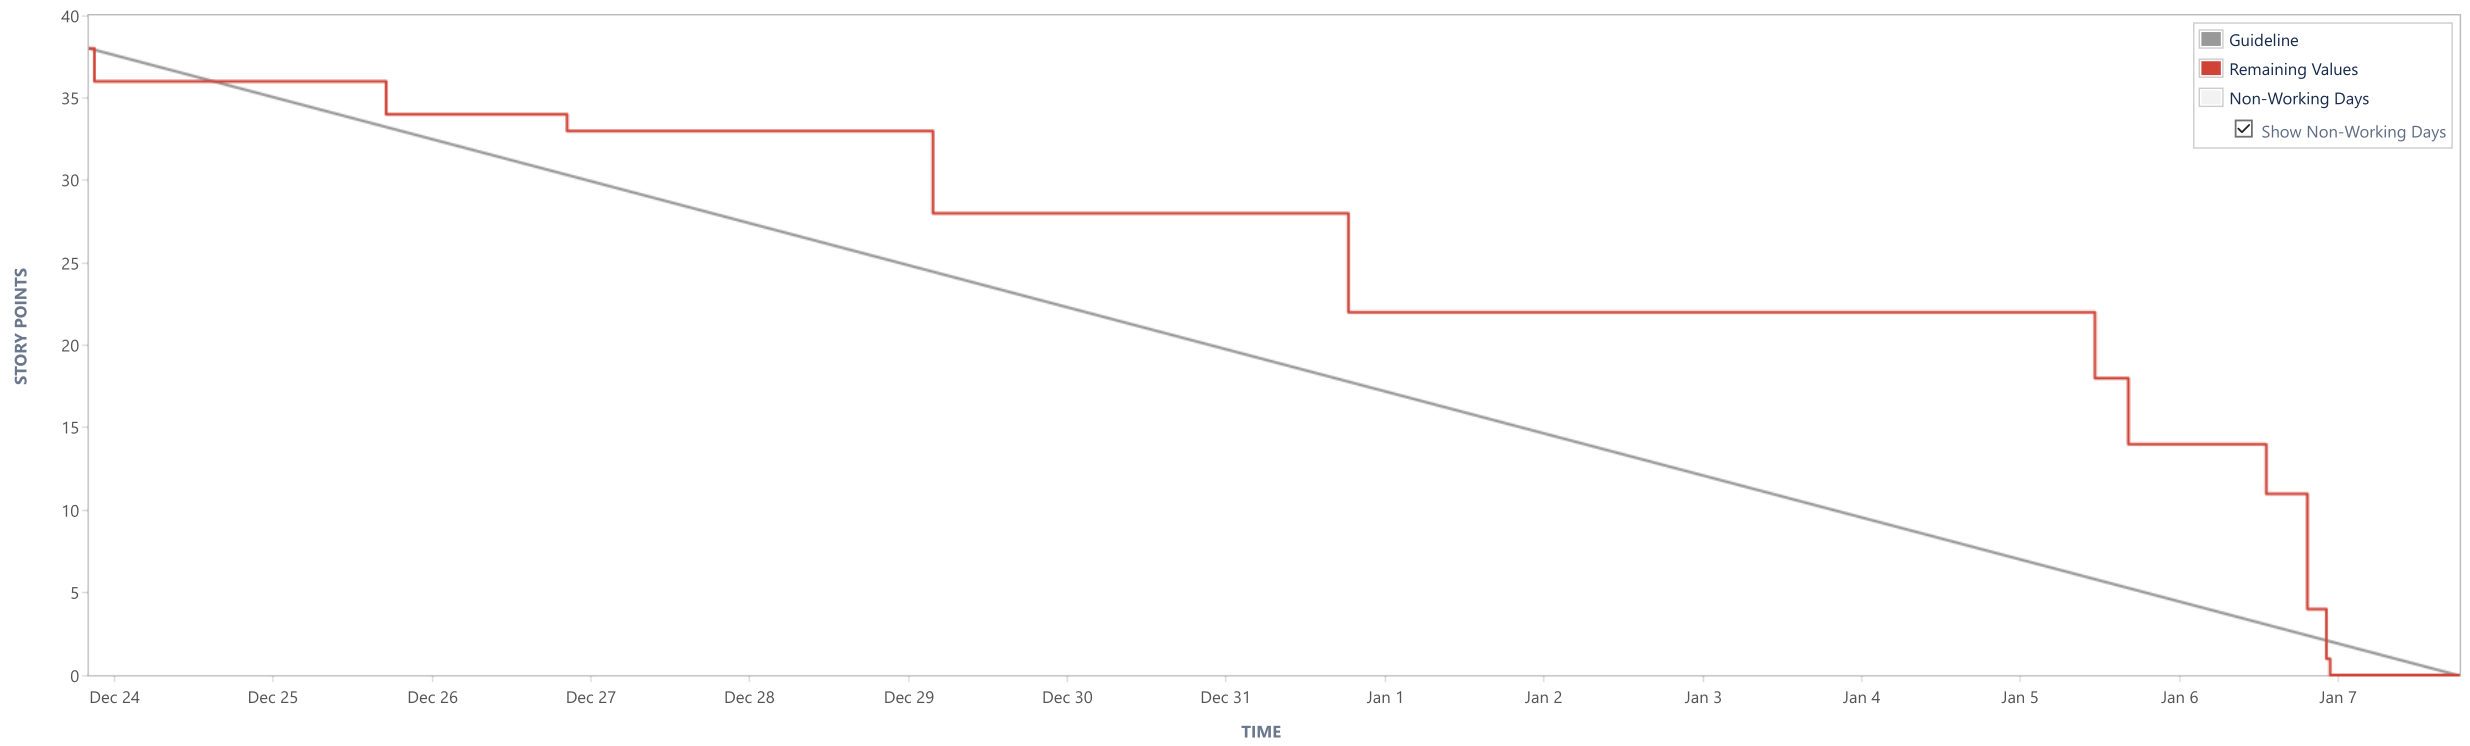
\includegraphics[width=\textwidth, height=5cm]{../img/sprint_03/Burndown-Sprint3.PNG}
        \caption{Burndown-Diagramm Sprint 3}
        \label{fig: Burndown-Sprint3}
    \end{figure}

    \noindent
    Zu Beginn des Sprints betrug der Gesamtaufwand des Sprints 38 Story Points.
    Dem Burn down Diagramm kann man entnehmen das wir unser Zeitmanagement verbessert haben.
    Storys wurden früher angefangen und fertiggestellt.
    Lediglich während der Weihnachtsfeiertage und über Neujahr wurden weniger Aufgaben erledigt.
    Der Sprint wurde am 07. Januar 2021 beendet und alle Storys wurden im vollen Umfang bearbeitet.



    \subsection{Sprintprobleme bzw. Hindernisse}

    Wie an dem obigen Burndowndiagramm zu erkennen ist, nahm die Velocity des Teams über die Weihnachtsfeiertage ab, was durchaus zu erwarten war. Dieser Umstand war dem gesamten Team bewusst und so wurde der Sprint passend geplant. Ab dem letzten Drittel des Sprints wurden die Tasks dann aber mit einem guten Tempo abgearbeitet, was sich in dem Burndowndiagramm widerspiegelt. So wurden dann auch alle Tasks, die im Umfang des Sprints enthalten waren, zwar spät aber dennoch fristgerecht beendet. Zusätzlich dazu, gab es Beschwerden über die Kommunikation über Discord. Jeder wird dazu angehalten öfter auf den Projekt Discord zu schauen um unnötige Verzögerungen zu vermeiden. In Verbindung dazu steht der Umstand, dass manche Reviews erst sehr spät nach bereits stehender PR bearbeitet wurden.

    \section{Erkenntnis aus der Retrospektive}

    Folgende Erkenntnisse ergaben sich aus der Retrospektive:\\

    \underline{Was lief gut?}
    \begin{itemize}
        \item Pairprogramming beibehalten
        \item Aktuelle Kommunikation und Hilfestellungen beibehalten
        \\
    \end{itemize}

    \underline{Was lief nicht so gut?}
    \begin{itemize}
        \item Teilweise noch viel Prokrastination
        \item Verzögerte Kommunikation durch seltenes Checken des Discords
        \\
    \end{itemize}

    \underline{Was sollte anders laufen?}
    \begin{itemize}
        \item Früher mit der ernsthaften Bearbeitung der Tasks starten
        \item Reviews so früh wie möglich durchführen
        \item Regelmäßig auf die Jira-Zeit achten und loggen
        \item Nach halbem Sprint generell Tasks PR-bereit
        \item Mehr Kommunikation ermöglicht schnellere Reviews und schnellere Hilfe
    \end{itemize}

    \section{Sonstige Anmerkungen}

    Da der Sprint um die Feiertagszeit herum datiert war, wurde dieser dementsprechend vom Umfang etwas niedriger als die vorherigen Sprints geplant. Dem Team war bewusst, dass vor allem in der Woche vom 24. Dezember 2020 bis zum 31. Dezember 2020 kein großer Fortschritt zu erwarten war. Das hat sich auch im Burndowndiagramm geäußert.


    \section{Fazit}
    Das Sprintziel \textit{\glqq Bugfixes, Vervollständigung vorhandener Features und Software präsentabel machen"} wurde erreicht und somit alle Tasks fristgerecht abgeschlossen. So wie der Sprint dem Umständen angepasst geplant war, wurde er zum größten Teil auch umgesetzt. Es war geplant, in der Zeit das Projekt von bekannten Bugs zu befreien und es generell in seinem aktuellen Zustand präsentabler zu machen. Dieses Ziel wurde auch durchaus erreicht.


\end{document}
